\chapter{Pérdida de energía en átomos pesados}
\label{chap:heavy}

%%%%%%%%%%%%%%%%%%%%%%%%%%%%%%%%%%%%%%%%%%%%%%%%%%%%%%%%%%%%%%%%%%%%%%%%
\section{Introducción}
%%%%%%%%%%%%%%%%%%%%%%%%%%%%%%%%%%%%%%%%%%%%%%%%%%%%%%%%%%%%%%%%%%%%%%%%
\label{sec:intro}

El estudio de procesos de pérdida de energía por impacto de iones 
en sólidos es una poderosa herramienta en diversas áreas de la ciencia
básica y tecnología de materiales. Para energías de impacto superiores 
a unos pocos keV/amu, las partículas cargadas monoenergéticas que 
penetran algún material pierden su energía a través de una serie de 
colisiones inelásticas consecutivas, principalmente con blancos
electrónicos~\cite{Chu:01,Sigmund:06}. La información proporcionada por 
el proceso de pérdida de energía es esencial no sólo para tener una 
mejor comprensión de la física detrás de las interacciones 
fundamentales, sino también porque es de vital importancia en muchos 
áreas aplicadas, tales como la implantación 
iónica~\cite{Creutzburg:19,Jeynes:16}, 
fusión~\cite{Mayer:20,He:17} y aplicaciones 
médicas~\cite{Schardt:10,AlcocerAvila:19,Vera:19}.

Tablas y códigos resultantes de aproximaciones semiempíricas están 
disponibles para una gran combinación de proyectiles y 
blancos~\cite{iaea_codes,Paul:03}. Sin embargo, el desarrollo de modelos
teóricos \textit{ab initio} son de crucial importancia para comprobar la 
fiabilidad de estas aproximaciones y determinar ciertos parámetros 
clave~\cite{Diwan:15,Damache:04,Damache:02} para la pérdida de energía 
media de iones por unidad de longitud de trayectoria $S(E)$. Los 
cálculos de dispersión inelástica de blancos pesados a partir de métodos 
basados en primeros principios constituyen una difícil tarea ya que 
resulta necesario tener en cuenta efectos 
relativistas~\cite{Montanari:09}. Estos efectos son importantes no sólo 
para definir el estado de los electrones internos sino también para 
determinar las energías de ligadura de las capas externas.

El método de Dirac--Fock (\acs{df}) es quizás la aproximación más 
conocida e implementada para describir la estructura en blancos 
relativistas. Esta aproximación se basa en el principio variacional y 
puede producir resultados muy precisos. Sin embargo, el principio 
variacional presenta varios inconvenientes: el precio de la precisión 
del método se paga con funciones de onda radiales dependientes de los 
términos, las cuales no son ortogonales entre configuraciones. Estas 
características hacen que el uso de las funciones de onda sea engorroso 
en el cálculo las transiciones radiativas y de colisión. Más aún, dado 
que el principio variacional implica la minimización de la energía 
total, las energías de transición entre niveles cercanos se obtienen 
como diferencias muy pequeñas entre números grandes, y los resultados 
son muy susceptibles a errores numéricos. Esto es especialmente 
importante para los átomos pesados porque la energía total es muy 
grande. 

En este Capítulo se estudia la estructura atómica de blancos pesados
y dos procesos de pérdida de energía de iones cuando inciden sobre 
ellos: potencia de frenado e ionización de capa $L$. En particular, se 
examinan tres grupos de elementos: metales de transición con capa de 
valencia $4d$, lantánidos con la capa $4f$ abierta y metales de 
transición pesados con la capa $4f$ llena. 

La modelo teórico que se usa para describir la estructura de los 
blancos atómicos relativistas se presenta en la 
Sección~\ref{sec:method-target}. El método está dado por la aproximación 
de potencial paramétrico desarrollada por Klapisch~\cite{Klapisch:77,
Klapisch:67,Klapisch:71,BarShalom:01}. En esta aproximación, el 
Hamiltoniano multielectrónico de Dirac se resuelve a partir de la 
combinación de la teoría de perturbaciones y la aproximación de campo 
central. Las funciones de onda del sistema se obtienen de la 
implementación del método de interacción de configuraciones~(\acs{ci}). 
La descripción precisa de los blancos relativistas requiere considerar 
configuraciones que influyen de manera significativa en el CI. Sin 
embargo, el cálculo de estructura en blancos de muchos electrones está 
computacionalmente limitado por la cantidad de electrones en las capas 
abiertas. Por lo tanto, se debe realizar una cuidadosa optimización de 
las configuraciones definidas. 

El enfoque teórico considerado para predecir los procesos de pérdida de 
energía en blancos relativistas se presenta en la 
Sección~\ref{sec:method-stopping}. El modelo combina diversas 
aproximaciones para tratar por separado la interacción del proyectil 
con, por un lado, los electrones de valencia y, por otro, los electrones 
ligados. Los electrones de conducción se describen a partir de un 
gas de electrones libres (FEG). Dos modelos diferentes se usan para 
describir el FEG: en la región de bajas energías, se usa el modelo de 
potencial apantallado con condición de cúspide 
(\acs{spcc})~\cite{Montanari:17} y, para energías alrededor del frenado 
máximo y valores superiores, se implementa el formalismo dieléctrico de 
Mermin-Lindhard (\acs{ml})~\cite{Mermin:70}. La aproximación de plasma 
local por capa~(\acs{slpa})~\cite{Montanari:13} describe la pérdida de 
energía debido a los electrones ligados. El modelo teórico requiere 
conocer las funciones de onda relativistas y energías de ligadura del 
blanco, considerando un cierto número de electrones de las capas 
externas en el FEG. Particularmente, la correcta descripción de blancos 
pesados que cuentan con electrones en la capa $4f$ es importante ya que 
estos electrones tiene un rol fundamental en la predicción de pérdida de 
energía a energías bajas~\cite{Roth:17}. 

En la Sección~\ref{sec:results-heavy} se presentan los resultados de 
este trabajo. Los cálculos de estructura atómica de nueve blancos 
pesados: Zr~(40), Nb~(41), Pd~(46), Gd~(64), Er~(68), Hf~(72), Ta~(73), 
Os~(76) y Pt~(78), se discuten en la 
Sección~\ref{subsec:results-target}. Los blancos relativistas se 
describen a partir de la resolución de la ecuación de Dirac en forma 
perturbativa. Las energías de enlace teóricas presentes se comparan con 
datos experimentales~\cite{Williams:95}. También se incluyen resultados 
de dos métodos teóricos: el método de 
Hartree--Fock~\cite{FroeseFischer:97} y de 
Dirac--Fock~\cite{Desclaux:73}. A partir de los valores teóricos 
obtenidos, en la Sección~\ref{subsec:FEG} se proponen parámetros del gas 
de electrones libres, que luego se usan en el cálculo de procesos de 
pérdida de energía. 
Las predicciones de pérdida de energía en tres blancos relativistas por 
impacto de iones se muestran y discuten en la 
Sección~\ref{subsec:results-stopping}. Se realizan comparaciones con 
datos experimentales en las regiones de energía disponibles. Los 
cálculos teóricos se comparan con los modelos teóricos de Grande y 
Schiwietz~\cite{Grande:01,casp52}, y de Sigmund y 
Schinner~\cite{DPASS20}. Debido a su gran implementación en diversas 
aplicaciones, se incluyen los valores semi-empíricos dados por el 
paquete SRIM-2013~\cite{Ziegler01} y las tablas ICRU-49~\cite{ICRU49}. 
Los cálculos de estructura atómica en blancos relativistas han sido 
publicados en la Ref.~\cite{Mendez:19relat}. Las secciones eficaces de 
potencia de frenado en Hf por impacto de protones fueron publicados en 
la Ref.~\cite{Montanari:20}. Se muestran resultados preliminares en Ta y 
Pt. Cálculos en Gd y Er se encuentran en preparación. Las conclusiones 
de este trabajo se presentan al final del Capítulo, en la 
Sección~\ref{sec:conclu-heavy}.

\begin{comment}
So far, only one experimental work has been published regarding the 
stopping power cross section of pure hafnium for 
protons~\cite{Sirotinin}, while more attention has been recently given 
to studies involving hafnium oxide due to its practical 
use~\cite{Abril,Behar,Primetzhofer,Roth}. It is well known that 
significant attention has been paid in recent years to transition 
metal-oxides such as HfO$_2$ because of their potential as alternative 
gate dielectrics to replace SiO$_2$ for the future generation of 
nano-electronics with less than 45 nm gate length~\cite{Choi,Robertson}. 
Some important physical properties of the above mentioned metal-oxide 
films depend on their thickness, which is often measured by using 
Rutherford Backscattering Spectrometry~\cite{Alfassi01,Tesmer01}. This 
method relies on the determination of both the scattering cross section 
and also the stopping power of ion beams in the material of interest.

In this study, we report experimental stopping power cross sections over 
the incident energy range (0.6-2.5) MeV for protons crossing 
self-supported Hf thin-film by using the transmission method. We aim not 
only to upgrade stopping power data compilations~\cite{HPaul03,mondim17} 
but also to provide useful information about the processes governing the 
slowing down of protons in multi-electronic targets. In the rare earth 
metals, the $4f$ electrons play an essential role in the stopping power 
since they belong to the first shell of bound electrons below the 
conduction band. As already noted \cite{Roth17}, the free electron gas 
(FEG) shows unexpected behavior in these elements, which casts doubts on 
its proper description. In the case of Hf, we found the contribution of 
the $4f$-shell to be decisive even at impact energies around the 
stopping maximum, as will be shown later.
\end{comment}


%%%%%%%%%%%%%%%%%%%%%%%%%%%%%%%%%%%%%%%%%%%%%%%%%%%%%%%%%%%%%%%%%%%%%%%%
\section{Descripción de blancos relativistas}
%%%%%%%%%%%%%%%%%%%%%%%%%%%%%%%%%%%%%%%%%%%%%%%%%%%%%%%%%%%%%%%%%%%%%%%%
\label{sec:method-target}

La descripción de los estados de átomos pesados relativistas se 
obtiene resolviendo el Hamiltoniano multielectrónico de 
Dirac~\cite{Klapisch:71,Klapisch:67,Klapisch:77,BarShalom:01}
\begin{equation}
 H = H' + H_{\mathrm{\mbox{\scriptsize Breit}}}(i,j) +
 H_{\mbox{\scriptsize QED}}\,,
\label{eq:htot}
\end{equation}
donde $H_{\mathrm{\mbox{\scriptsize Breit}}}(i,j)$ es el término de 
Breit, $H_{\mbox{\scriptsize QED}}$ considera los efectos 
electrodinámicos cuánticos (\acs{qed}), y
\begin{equation}
 H' = \sum_i \left[ h_i^{\mbox{\scriptsize D}} - \frac{Z}{r_i}\right]
 + \sum_{i<j}\frac{1}{r_{ij}}\,,
\label{eq:HDirac}
\end{equation}
siendo $h_i^{\mbox{\scriptsize D}}$ el término cinético del 
Hamiltoniano de Dirac de una partícula. Los términos restantes en la
Ec.~(\ref{eq:HDirac}) corresponden a las interacciones 
núcleo--electrón y electrón--electrón, respectivamente. A partir de la 
aproximación de campo central, e introduciendo un potencial paramétrico 
$U(\boldsymbol{\alpha},r)$, el Hamiltoniano $H'$ se puede escribir como 
la combinación de un término de orden cero, 
\begin{equation}
 H_0 = \sum_i h_i^{\mbox{\scriptsize D}} + U(\boldsymbol{\alpha},r_i)\,,
\end{equation}
más una pequeña perturbación
\begin{equation}
 H_1 = \sum_{i<j}\frac{1}{r_{ij}}
 - \sum_i \left[ \frac{Z}{r_i} + U(\boldsymbol{\alpha},r_i) \right]\,.
\end{equation}
Las soluciones de espinor de cuatro componentes de un electrón 
$\varphi_{nljm}(\mathbf{r})$, de la ecuación de Dirac
\begin{equation}
\left[ h_i^{\mbox{\scriptsize D}} +U(\boldsymbol{\alpha},r) \right] 
\varphi_{nljm}(\mathbf{r}) 
= \varepsilon_{nljm} \varphi_{nljm}(\mathbf{r})\,,
\label{eq:ecuacionDirac}
\end{equation}
se denominan orbitales relativistas y se caracterizan por un conjunto de 
números cuánticos $nljm$, donde $l$ es el número cuántico del momento 
angular orbital de la componente fuerte del orbital.

La solución de orden cero de un sistema $N$--electrónico se construye a 
partir de productos antisimetrizados de orbitales en cualquier esquema 
de acoplamiento elegido $\Gamma JM$ como 
\begin{equation}
\Psi_{\Gamma}\left(\mathbf{r}_1,\mathbf{r}_2,\ldots,\mathbf{r}_N\right)
=\mathcal{A}\sum_{all\,\,m}\left\langle\Gamma JM\mid m_1 m_2,\ldots,m_{N}\right
\rangle \prod_{a} \varphi_{n_a l_a j_a m_a}\left(\mathbf{r}_a\right)\,,
\end{equation}
donde $\mathcal{A}$ es el operador de antisimetría. Los estados y niveles 
específicos se denotan $\Gamma_iJ_iM_i$ y $\Gamma_iJ_i$, respectivamente,
donde $\Gamma_i$ representa el conjunto de números cuánticos necesario 
para identificar el estado de manera únivoca. 

Una configuración 
$C\equiv\prod_{a=1}^N\mathbf{j}_a=\prod_{i=1}\mathbf{j}_i^{q_i}$ es un 
conjunto de estados degenerados, con valores fijos 
$\mathbf{j}_i=n_il_ij_i$
y números de ocupación $q_i$, todos con energías de orden cero 
$E_C^0=\prod_{i=1}\,q_i\varepsilon_i$. 
El Hamiltoniano $H'$ se construye sobre la base de las configuraciones 
elegidas obtenidas con el potencial paramétrico. Luego, la matriz es 
diagonalizada, produciendo estados de configuración mixtos y energías 
de primer orden con algunas correcciones de correlación. Las funciones 
de onda resultantes se utilizan para agregar las correcciones QED y el 
término de Breit a las energías como perturbaciones de segundo orden.

La idea detrás del potencial paramétrico $U(\boldsymbol{\alpha},r)$
\cite{Klapisch:77} es describir de manera simple el apantallamiento de 
la distribución de carga de los electrones usando una expresión 
paramétrica analítica, donde 
$\boldsymbol{\alpha}=\left\{\alpha_1,\alpha_2,\ldots,\alpha_k\right\}$ 
es un conjunto de parámetros que se definen mediante la optimización 
del sistema y $k$ es el número de capas ocupadas. Aplicando la ecuación 
de Poisson a la densidad de carga radial de los $q$ electrones descritos 
por orbitales de tipo Slater se tiene que
\begin{equation}
\rho(r) = -4\pi r^2 qN\left|r^{l+1}e^{-\alpha r/2}\right|^2\,,
\end{equation} 
con condiciones de borde tal que
\begin{equation}
U(\boldsymbol{\alpha},r\rightarrow\infty)=Z-\frac{q}{r}\,.
\end{equation} 
Aquí, $N$ es un factor de normalización, y $\alpha_i$ está relacionado 
con el radio medio de la capa tal que $\alpha_i=(2l+3)/\langle r\rangle_i$. 
Es necesario mostrar que el potencial para diversas capas y el núcleo 
se puede escribir como
\begin{equation}
U(\boldsymbol{\alpha},r)=-\frac{1}{r} \left[I+\sum_s q_s\, g(L_s,\alpha_s,r) 
+ \sum_t q_t\,f(l_t,\alpha_t,r)\right]\,,
\label{eq:potparam}
\end{equation}
donde los índices $s$ y $t$ recorren las capas cerradas y abiertas, 
respectivamente. El valor $I$ es el grado de ionización más uno. 
%Esto elimina la auto-interacción adicional de los electrones ligados. 
%Aquí, $\boldsymbol{\alpha}$ representa un conjunto de parámetros 
%$\left\{\alpha_s,\alpha_t\right\}$ que describen el radio medio de las 
%capas. 
Las funciones $f$ y $g$ son tales que
\begin{eqnarray}
f(l,\alpha,r)&=&\mathrm{e}^{-\alpha r}\sum_{j=1}^{2l+1}
\left(1-\frac{j}{2l+2}\right)\frac{(\alpha r)^j}{j!}\,,\\
g(L,\alpha,r)&=&\frac{1}{2n^2}\sum_{l=0}^{L=n-1}
(4l+2)f\left(l,\alpha^{(l)},r\right)\,,
\end{eqnarray}
donde $n$ es el número cuántico principal y $\alpha^{(l)}$ incluye una
corrección para la ligera diferencia en el radio debido al número del
momento angular cuántico de las subcapas. 
Los parámetros libres $q$ son el número efectivo de electrones en la 
capa y satisfacen $I+\sum_s q_s+\sum_t q_t=Z$. 

Esta parametrización resulta en que cualquier cantidad atómica calculada 
con las funciones de onda dadas por la Ec.~(\ref{eq:ecuacionDirac}) 
junto con el potencial~(\ref{eq:potparam}) se convierte en una función 
numérica de los parámetros. Hay múltiples formas posibles de elegir los 
parámetros $\boldsymbol{\alpha}$, de acuerdo a diversos criterios 
teóricamente válidos. Entre ellos, se destacan tres;
\begin{itemize}
\item criterio espectroscópico: minimización de la desviación \acs{rms} 
entre los niveles de energía teóricos y experimentales,
\item criterio variacional: minimización de la energía total, y
\item criterio perturbacional: minimización del Hamiltoniano perturbativo
$H_1$. 
\end{itemize}
En este trabajo, se implementa la minimización de las energías de 
configuración promedio, o de las energías de cualquier conjunto de 
niveles elegido. Dado que las energías de primer orden sobre las que 
actúa la optimización incluyen la contribución de intercambio exacta, 
los parámetros resultantes absorben el efecto del intercambio y, por lo 
tanto, no hay necesidad de un potencial de intercambio adicional 
explícito.

Por otro lado, siendo $U(\boldsymbol{\alpha},r)$ un potencial central,
es posible plantear la separación de variables esféricas de las 
soluciones de la ecuación de Dirac~(\ref{eq:ecuacionDirac}), tal que
\begin{equation}
\varphi_{nljm}(\mathbf{r}) = \frac{1}{r} \left( 
\begin{array}{c}
i P_{nlj}(r) \,\Omega_{jlm}(\hat{\mathbf{r}}) \\ 
- Q_{nlj}(r) \,(\boldsymbol{\sigma}\cdot\hat{\mathbf{r}})\,
\Omega_{jlm}(\hat{\mathbf{r}})
\end{array}
\right)\,,
\label{eq:sepespinor}
\end{equation}
donde $P_{nlj}(r)$ y $Q_{nlj}(r)$ son las componentes fuerte y débil de 
los espinores de Dirac, respectivamente. Los espinores esféricos 
$\Omega_{jlm}(\hat{\mathbf{r}})$ son autoestados de $J^2$ y $J_z$ a 
través de la relación
\begin{equation}
\Omega_{j,l,m}(\theta,\phi)=\sum_{\mu} C(l,1/2,j;m-\mu,\mu,m) 
Y_{l,m-\mu}(\theta,\phi)\chi_{\mu}\,,
\end{equation}
donde $C\left(j_1,j_2,j;m_1,m_2,m\right)$ son los coeficientes de 
Clebsch--Gordan. Así, el valor esperado de cualquier operador $\hat{A}$ 
está dado por
\begin{equation}
\langle\hat{A}\rangle=\int_0^{\infty}\left[P^*(r)\,\hat{A}\,P(r) 
 +Q^*(r)\,\hat{A}\,Q(r)
\right]\,dr\,.
\label{eq:meanvalr}
\end{equation}
Para los orbitales radiales, se usa la notación $nl\pm$, que significa 
$nlj$, donde el índice $j=l\pm1/2$ se representa como $\pm$.

El método del potencial paramétrico desarrollado por Klapisch derivó en
el paquete de códigos \textsc{hullac}~\cite{BarShalom:01} y constituye 
el estado del arte en el cálculo de estructura y colisiones en iones de 
carga múltiple. Además, \textsc{hullac} fue el primer programa que 
permitió realizar espectroscopía de plasmas y resolver espectros de 
blancos complejas con varias capas internas abiertas. Existen otras 
metodologías, y sus respectivas implementaciones numéricas, que no se 
verán aquí. Por ejemplo, el código \textsc{grasp}~\cite{Grant:80} se 
basa en el método de Dirac--Fock mientras que el 
código~\textsc{fac}~\cite{Gu:08} también implementa un potencial 
efectivo paramétrico.

%%%%%%%%%%%%%%%%%%%%%%%%%%%%%%%%%%%%%%%%%%%%%%%%%%%%%%%%%%%%%%%%%%%%%%%%
\section{Modelo teórico de pérdida de energía}
%%%%%%%%%%%%%%%%%%%%%%%%%%%%%%%%%%%%%%%%%%%%%%%%%%%%%%%%%%%%%%%%%%%%%%%%
\label{sec:method-stopping}

Cuando un ion energético penetra en un material, éste pierde energía 
cinética a lo largo del camino recorrido debido a colisiones con los 
núcleos y electrones del blanco. La pérdida de energía promedio 
por unidad de longitud de trayectoria se conoce como potencia de frenado 
$S=dE/dx$ del blanco debido a un proyectil específico. Es conveniente 
normalizar la potencia de frenado $S(E)$ por la densidad atómica $n$ 
del blanco para eliminar la dependencia de la naturaleza del material. 
La cantidad resultante se conoce comúnmente como sección eficaz de 
frenado, $\epsilon=S/n$. 

La pérdida de energía de iones en blancos metálicos responde a 
diferentes mecanismos físicos, dependiendo de la velocidad del proyectil 
incidente. A bajas velocidades, las colisiones binarias son responsables 
de la pérdida de energía y la contribución principal está dada por la 
ionización de los electrones de la banda de conducción del metal. En 
general, estos electrones se describen a partir de un gas de electrones 
libres de velocidad de Fermi, $v_F$. Sin embargo, por arriba de un valor 
particular de velocidad (i.e., $v\geq 1.5\,v_F$), no sólo ocurren 
excitaciones binarias sino también colectivas (plasmones), que deben ser
consideradas~\cite{Montanari:17}. En la región de altas energías, la 
contribución a la pérdida de energía de los electrones ligados se vuelve
significativa y también se debe incluir en el modelo.

El método teórico de pérdida de energía que se implementa aquí combina 
tres metodologías distintas para modelar la interacción del blanco con 
el proyectil incidente. Por un lado, los electrones de valencia (o 
conducción) se describen como un gas de electrones libres. A bajas 
energías, esta interacción se describe a partir del modelo de potencial
apantallado con condición de cúspide (\acs{spcc}), desarrollado por 
Montanari y Miraglia~\cite{Montanari:17}. En la región de energías donde 
la contribución del plasmón es esencial, el FEG se modela mediante el 
formalismo dieléctrico de Mermin-Lindhard (ML)~\cite{Mermin:70}, que 
considera las excitaciones colectivas y binarias. Finalmente, la 
interacción del proyectil y los electrones ligados se describe 
implementando la aproximación de plasma local por capa 
(\acs{slpa}), también desarrollada por Montanari y 
Miraglia~\cite{Montanari:17,Montanari:13}. A continuación se describen 
brevemente cada uno de estas metodologías. 

El modelo SPCC está basado en la aproximación de colisión binaria no 
perturbativa, de manera que es válida para valores de energías menores a 
las excitaciones de plasmones. La SPCC se basa en un potencial centrado 
apantallado con una condición de cúspide para la densidad electrónica 
cerca del proyectil (ver Apéndice~\ref{app:SPCC}). Este modelo ha 
probado dar buenas descripciones para la densidad de electrones inducida, 
aún para proyectiles con carga negativa~\cite{Montanari:17}. 
Además, predice correctamente las diferencias entre protón-antiprotón en 
la potencia de frenado, más conocido como el efecto Barkas. El 
formalismo SPCC depende sólo del radio de Wigner-Seitz $r_S$, que es una 
medida de la densidad electrónica del FEG. Para metales de $r_S$ 
conocidos, el SPCC describe correctamente los valores experimentales de 
la potencia de frenado a bajas energías~\cite{Montanari:17}, en 
concordancia con resultados DFT de Echenique y 
colaboradores~\cite{Echenique:81,Nagy:89} a $v=0$.

El formalismo dieléctrico de ML es una aproximación perturbativa de 
respuesta lineal, que depende del cuadrado de la carga del proyectil 
(ver Apéndice~\ref{app:ML}). En este formalismo, la respuesta de los 
electrones del blanco al paso de iones se describe a través de la 
función dieléctrica cuántica, que depende de los parámetros 
característicos del FEG. Este modelo es válido a partir de cierto valor 
umbral de velocidad de impacto $v_P$ en la excitación de plasmones 
(alrededor del máximo de la sección eficaz de frenado). En el formalismo 
dieléctrico, este valor se puede obtener como 
$v_P\,\approx\,v_F[1+(3\pi\,v_F)^{-1/2}]$~\cite{suppression}. 
%Para describir la pérdida de energía considerando la excitación colectiva y 
%binaria, se recurre al formalismo dieléctrico de Mermin-Lindhard 
%(ML)~\cite{Mermin:70}, que es una aproximación perturbativa de respuesta 
%lineal, por lo que depende del cuadrado de la carga del proyectil 
%(ver Apéndice~\ref{app:ML}). En este formalismo, la respuesta de los 
%electrones del blanco al paso de iones se describe a través de la 
%función dieléctrica cuántica, que depende de los parámetros 
%característicos del FEG.

El método SLPA también se basa en un formalismo dieléctrico, que trata 
por separado la respuesta dieléctrica de cada capa $nl$ (ver 
Apéndice~\ref{app:SLPA}). Este modelo sólo depende de las densidades 
radiales orbitales del estado fundamental del blanco y sus energías de 
ligadura. El modelo incluye los procesos colectivos y el apantallamiento 
entre electrones. Particularmente, la contribución de los electrones 
ligados a la sección eficaz de frenado total considera las 
contribuciones independientes de cada subcapa. 

%%%%%%%%%%%%%%%%%%%%%%%%%%%%%%%%%%%%%%%%%%%%%%%%%%%%%%%%%%%%%%%%%%%%%%%%
\section{Resultados}
%%%%%%%%%%%%%%%%%%%%%%%%%%%%%%%%%%%%%%%%%%%%%%%%%%%%%%%%%%%%%%%%%%%%%%%%
\label{sec:results-heavy}

En esta Sección se presentan los resultados de estructura atómica de 
nueve blancos relativistas: Zr, Nb, Pd, Gd, Er, Hf, Ta, Os y Pt, a 
partir de la implementación del método de potencial paramétrico y la
optimización de las configuraciones electrónicas que se incluyen el CI.
También se presentan resultados de pérdida de energía por unidad de 
longitud de trayectoria (potencia de frenado) en tres blancos 
relativistas: Hf, Ta y Pt. Tanto los cálculos de estructura atómica como 
las predicciones de pérdida de energía que se presentan aquí han sido 
publicados y se encuentran en las 
Refs.~\cite{Mendez:19relat,Montanari:20}. 

%=======================================================================
\subsection{Energías de ligadura y valores medios}
%=======================================================================
\label{subsec:results-target}

Los efectos de la interacción de configuraciones son muy importantes en 
el caso de los átomos relativistas. Así, la correcta descripción del 
blanco depende de las configuraciones consideradas en la CI. En esta 
Sección, la optimización de los blancos consiste en determinar las 
configuraciones que contribuyen de manera significativa a la mezcla en 
la interacción de configuraciones. 

El Hamiltoniano perturbativo de Dirac, dado por la Ec.~(\ref{eq:HDirac}), 
de los blancos relativistas a describir se resuelve aplicando el método 
perturbativo descrito anteriormente. Por simplicidad, llamamos a este 
método Dirac perturbativo (PD). Las soluciones numéricas se obtienen 
usando el paquete de códigos {\sc hullac}~\cite{BarShalom:01}. En este 
conjunto de programas computacionales, el código {\sc relac} permite 
calcular las energías de ligadura relativistas y funciones de onda 
orbitales.

\begin{table}[t]
\centering
\begin{tabular}{
>{\centering\arraybackslash}p{0.12\textwidth}
>{\centering\arraybackslash}p{0.14\textwidth}
>{\centering\arraybackslash}p{0.14\textwidth}
>{\centering\arraybackslash}p{0.08\textwidth}
>{\centering\arraybackslash}p{0.36\textwidth}}
\rowcolor{mydarkgray} 
Grupo & Nombre    & Símbolo & $Z$ & Configuración fundamental \\
 
I      & Circonio  & Zr      & 40  & [Kr]~$4d^2\,5s^2$ \\
\rowcolor{mygray} 
       & Niobio    & Nb      & 41  & [Kr]~$4d^4\,5s^1$ \\
       & Paladio   & Pd      & 46  & [Kr]~$4d^{10}$ \\
\rowcolor{mygray} 
II     & Gadolinio & Gd      & 64  & [Xe]~$4f^7\,5d\,6s^2$ \\
       & Erbio     & Er      & 68  & [Xe]~$4f^{12}\,6s^2$ \\
\rowcolor{mygray} 
III    & Hafnio    & Hf & 72 & [Xe]~$4f^{14}\,5d^2\,6s^2$ \\
       & Tántalo   & Ta & 73 & [Xe]~$4f^{14}\,5d^3\,6s^2$ \\
\rowcolor{mygray} 
       & Osmio     & Os & 76 & [Xe]~$4f^{14}\,5d^6\,6s^2$ \\
       & Platino   & Pt & 78 & [Xe]~$4f^{14}\,5d^9\,6s$ \\
\end{tabular}
\caption[Blancos relativistas y sus configuraciones fundamentales]
{Blancos relativistas: símbolos, cargas nucleares $Z$, configuraciones 
fundamentales y serie.}
\label{tab:gruposrelat} 
\end{table}

Los elementos que examinamos en esta Sección se dividen en tres grupos 
según la serie y período de la tabla periódica al que pertenecen. Los 
blancos a estudiar, sus símbolos, carga nuclear $Z$ y configuraciones 
fundamentales se muestran en la Tabla~\ref{tab:gruposrelat}. El grupo A
está compuesto por metales de transición del período 5: circonio, niobio
y paladio. En el grupo B se incluyen lantánidos del período 6: 
gadolinio y erbio. Finalmente, el grupo C se compone metales de 
transición del período 6: hafnio, tántalo, osmio y platino.

Se puede escribir una fórmula general para la configuración fundamental 
de los metales de transición como
\begin{equation}
[\text{X}]\,nd^w\,(n+1)s^x\,,
\end{equation}
donde X es la configuración electrónica del gas noble más cercano, para 
el grupo A: $n=4$, $w=2,4,10$ y $x=2,1,0$ y para el grupo C: $n=5$, 
$w=2,3,6,9$ y $x=2,2,2,1$. Los electrones $nd$ y $(n+1)s$ tienen 
energías de ligadura similares. Por lo tanto, las configuraciones 
\begin{gather}
nd^w(n+1)s^2,
\label{eq:confsmtran1} \\
nd^{w+1}(n+1)s,
\label{eq:confsmtran2} \\
nd^{w+2}
\label{eq:confsmtran3}
\end{gather}
tienen energías comparables. Dado que las configuraciones de la 
Ec.~(\ref{eq:confsmtran1}), (\ref{eq:confsmtran2}) y 
(\ref{eq:confsmtran3}) tienen la misma paridad, éstas cumplen los dos 
requerimientos mencionados anteriormente, y son fundamentales en los 
cálculos de mezcla de configuraciones. Así, por ejemplo, para el átomo 
de Zr, cuyo estado fundamental está dado por [Kr]~$4d^2\,5s^2$, se 
incluyen las configuraciones $4d^2\,5s^2$, $4d^3\,5s$ y $4d^4$. 
Similarmente, para el átomo de Pt, las configuraciones [Xe]~$5d^9\,6s$ y 
$5d^{10}$ son consideradas en el cálculo relativista.

Por otro lado, la fórmula general para la configuración fundamental de 
los lantánidos está dada por
\begin{equation}
nf^w\,(n+1)d^x\,(n+2)s^y\,,
\end{equation}
donde $n=4$, $w=7,12$, $x=1,0$ y $y=2,2$. En el caso de Gd, también 
se deben incluir las interacciones entre los electrones de las capas
$4f$ y $5d$, que están abiertas. Así, las contribuciones más 
importantes a la interacción de configuraciones están dadas por la 
mezcla de las configuraciones $4f^7\,5d\,6s^2$ y $4f^8\,6s^2$.
Para Er, la mayor mezcla es producida por las configuraciones 
$4f^{12}\,6s^2$ y $4f^{12}\,5d\,6s$.

\begin{figure}
\centering
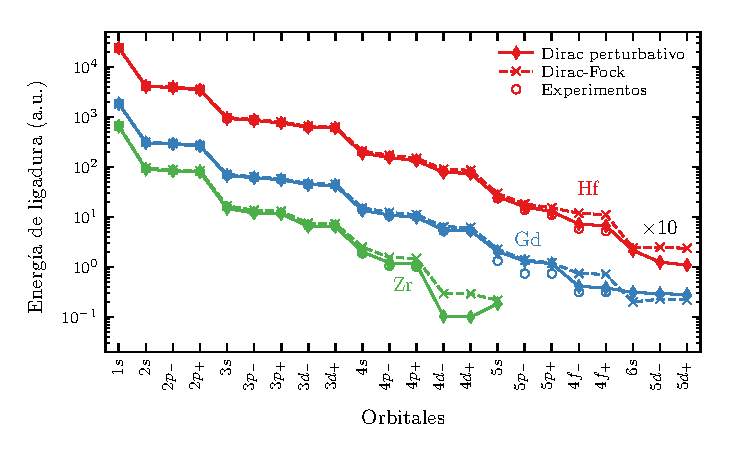
\includegraphics[width=\textwidth]{heavy/bindenerA.eps} 
\caption[Energías de ligadura de blancos relativistas]
{Energías de ligadura de Zr, Nb, Gd, Er, Hf y Ta. Símbolos: 
$\blacklozenge$ resultados teóricos del presente trabajo, 
$\triangleleft$ valores teóricos del método 
Dirac--Fock~\cite{Desclaux:73}, $\times$ valores teóricos según 
Hartree--Fock, y $\medcircle$ datos experimentales en 
sólidos~\cite{Williams:95}.}
\label{fig:bindenerA}
\end{figure}

\begin{figure}
\centering
\includegraphics[width=\textwidth]{heavy/bindenerB.eps} 
\caption[Energías de ligadura de blancos relativistas]
{Energías de ligadura de Pd, Gd, Er y Pt. Símbolos: $\blacklozenge$ 
resultados teóricos del presente trabajo, $\triangleleft$ valores 
teóricos del método Dirac--Fock~\cite{Desclaux:73}, $\times$ valores 
teóricos según Hartree--Fock, y $\medcircle$ datos experimentales en 
sólidos~\cite{Williams:95}.}
\label{fig:bindenerB}
\end{figure}

Las energías de ligadura de los blancos relativistas de la 
Tabla~\ref{tab:gruposrelat} que se obtienen a partir del método PD se 
dan en la Tabla~\ref{tab:relatresults}. También se incluyen los valores 
medios $\langle r\rangle$ de cada capa, los cuales se obtienen a partir 
de la Ec.~(\ref{eq:meanvalr}). Los resultados teóricos PD se muestran en 
las Figs.~\ref{fig:bindenerA} y \ref{fig:bindenerB} con símbolos 
$\blacklozenge$. Se incluyen valores experimentales de los blancos en 
estado sólido~\cite{Williams:95}, que se presentan con símbolos 
$\medcircle$. Los resultados obtenidos por Desclaux~\cite{Desclaux:73} 
mediante la implementación del método de Dirac--Fock se ilustran con 
símbolos $\triangleleft$. Además, se incluyen resultados no relativistas 
obtenidos mediante la implementación del método de 
Hartree--Fock~\cite{FroeseFischer:97} (símbolos $\times$). Los valores 
de energía correspondientes a Os y Er se muestran multiplicados por un 
factor 10 para tener mayor claridad en las figuras. Las líneas 
verticales de la figura esquematizan la separación entre los electrones 
ligados y el gas de electrones libres que considera el modelo de pérdida 
de energía. Las líneas horizontales ilustran los valores de energía de 
Fermi del FEG. Estos valores se  discuten más adelante, en la 
Sección~\ref{subsec:FEG}.

Dado que en las Figs.~\ref{fig:bindenerA} y~\ref{fig:bindenerB} las 
energías de enlace varían en un rango de cinco órdenes de magnitud, no 
es posible discernir las discrepancias entre los datos experimentales y 
los resultados teóricos obtenidos mediante los métodos de Hartree--Fock, 
Dirac--Fock y Dirac perturbativo. Para poder inspeccionar estas 
diferencias con más detalle, en la Fig.~\ref{fig:ratios} se calculan las 
relaciones entre las energías de ligadura experimentales 
$E^{\mbox{\scriptsize exp}}$ y teóricas (HF, DF y PD). A grandes rasgos,
la figura muestra que las correcciones relativistas son críticas para 
describir la estructura atómica de los blancos considerados, incluso 
para las capas externas. 

\begin{figure}
\centering
\includegraphics[width=\textwidth]{heavy/ratios_heavy_barh.eps} 
\caption[Razón $E^{\mbox{\scriptsize exp}}/E$ entre energías de ligadura 
experimentales y teóricas.]
{Razón $E^{\mbox{\scriptsize exp}}/E$ entre energías de ligadura 
experimentales y teóricas de los blancos de la 
Tabla~\ref{tab:gruposrelat}: métodos de Hartree--Fock (barras gris 
oscuro), Dirac--Fock (barras gris claro), y Dirac perturbativo (barras 
de colores).}
\label{fig:ratios}
\end{figure}

Como es de esperarse, el método HF (barras gris oscuro) es insuficiente 
para describir tanto la estructura interna. Sin embargo, también falla 
en la descripción de las capas externas del blanco. Por ejemplo, la 
energía de enlace no relativista de la subcapa $4f$ del Er es cuatro 
veces el valor experimental. Discrepancias de esta magnitud conduce a la 
subestimación de la ionización de los electrones $4f$, desplazando el 
umbral a energías más altas. Sin embargo, nótese que para los blancos 
más pesados ($Z\ge 64$), las desviaciones disminuyen significativamente 
en la región media ($n=3$) de la estructura. En promedio, el método HF 
proporciona una desviación de los valores experimentales del 20\%, con 
errores relativos máximos en las capas de valencia de hasta 300\%. Así, 
la inclusión de correcciones relativistas es necesaria en estos blancos.

Efectivamente, los valores teóricos relativistas Dirac--Fock (barras 
gris claro) mejoran la descripción de las capas internas de los blancos 
de forma sistemática. Sin embargo, las discrepancias con los valores 
experimentales en las capas cercanas a la banda de valencia siguen 
siendo significativas. Nótese que la descripción DF reduce las 
desviaciones de las capas más externas pero en todos los casos mantiene 
la misma relación que HF con los valores experimentales. Este 
comportamiento es atribuible a la metodología variacional que ambos 
implementan, donde los errores en la descripción de las capas internas 
se propagan hacia las más externas. En promedio, este método variacional 
relativista presenta errores relativos del 16\%, con dispersiones 
máximas del 175\%. 

El acuerdo entre los resultados teóricos perturbativos relativistas de 
este trabajo (barras de color) y las mediciones experimentales es en 
general muy bueno. Las energías de enlace obtenidas para los blancos del 
grupo A es del 4\%, a excepción de las capas $4p\pm$ del Zr y Nb. Los 
lantánidos del grupo B muestran un acuerdo por debajo del 3\%, salvo las 
subcapas más externas $5s$, $5p$ y $4f$ del Gd. Asimismo, los resultados 
teóricos PD de los metales de transición del grupo C coinciden con los 
valores experimentales en hasta 3\%, excepto las subcapas $5p$ y $4f$ de 
Hf y Ta. En todos los casos, los resultados obtenidos a partir del 
método perturbativo describen los datos experimentales con mayor 
precisión que los valores dados por el método variacional de 
Hartree--Fock~\cite{FroeseFischer:97} y su versión 
relativista~\cite{Desclaux:73}. En general, el método perturbativo 
permite describir en forma más precisa tanto las capas más internas 
--donde se esperan los efectos relativistas-- como las capas externas.
%A diferencia de los métodos HF y DF, el método PD incluye efectos de 
%correlación electrónica mediante la interacción de configuraciones. En 
%estos blancos, la inclusión de estos efectos es tan necesaria como las
%correcciones relativistas.

\vspace{0.5cm}
\begin{tabularx}{\textwidth}{
>{\centering\arraybackslash}p{0.04\textwidth}
>{\centering\arraybackslash}p{0.075\textwidth}
>{\centering\arraybackslash}p{0.075\textwidth}
>{\centering\arraybackslash}p{0.075\textwidth}|
>{\centering\arraybackslash}p{0.075\textwidth}
>{\centering\arraybackslash}p{0.075\textwidth}
>{\centering\arraybackslash}p{0.075\textwidth}|
>{\centering\arraybackslash}p{0.075\textwidth}
>{\centering\arraybackslash}p{0.075\textwidth}
>{\centering\arraybackslash}p{0.075\textwidth}}
\captionsetup{width=\linewidth}
\caption[Energías de ligadura y valores $\langle r \rangle$ de blancos
relativistas]
{Energías de ligadura teóricas y experimentales~\cite{Williams:95} de 
los elementos de la Tabla~\ref{tab:gruposrelat}. Valores medios 
$\langle r \rangle$ en a.u. obtenidos a partir de la 
Ec.~(\ref{eq:meanvalr}).}
\label{tab:relatresults}\\
\rowcolor{mydarkgray} 
$nl\pm$ & 
$E^{\mathrm{exp}}$ & $E^{\mathrm{PD}}$ & $\langle r\rangle^{\mathrm{PD}}$ &
$E^{\mathrm{exp}}$ & $E^{\mathrm{PD}}$ & $\langle r\rangle^{\mathrm{PD}}$ &
$E^{\mathrm{exp}}$ & $E^{\mathrm{PD}}$ & $\langle r\rangle^{\mathrm{PD}}$ \\
\endfirsthead
\caption*{Tabla 4.2 (Cont.): 
Energías de ligadura teóricas y experimentales~\cite{Williams:95} de 
los elementos de la Tabla~\ref{tab:gruposrelat}. Valores medios 
$\langle r \rangle$ en a.u. se obtienen a partir de la 
Ec.~(\ref{eq:meanvalr}).} \\ \rowcolor{mydarkgray} 
$nl\pm$ & 
$E^{\mathrm{exp}}$ & $E^{\mathrm{PD}}$ & $\langle r \rangle^{\mathrm{PD}}$ &
$E^{\mathrm{exp}}$ & $E^{\mathrm{PD}}$ & $\langle r \rangle^{\mathrm{PD}}$ &
$E^{\mathrm{exp}}$ & $E^{\mathrm{PD}}$ & $\langle r \rangle^{\mathrm{PD}}$ \\
\endhead
\endfoot
\endfoot
      & \multicolumn{3}{c}{Zr}   & \multicolumn{3}{c}{Nb}   & \multicolumn{3}{c}{Pd} \\
\rowcolor{mygray} 
$1s$  & 661.41 & 651.34 & 0.0372 & 697.72 & 685.57 & 0.0362 & 894.85 & 880.77 & 0.032 \\
$2s$  & 93.05  & 90.40  & 0.163  & 99.15  & 95.94  & 0.159  & 132.4  & 128.7  & 0.138 \\\rowcolor{mygray} 
$2p-$ & 84.78  & 82.78  & 0.139  & 90.59  & 87.85  & 0.136  & 122.4  & 119.7  & 0.117 \\
$2p+$ & 81.69  & 79.66  & 0.144  & 87.13  & 84.40  & 0.140  & 116.6  & 113.9  & 0.122 \\\rowcolor{mygray} 
$3s$  & 15.81  & 14.76  & 0.460  & 17.15  & 16.08  & 0.445  & 24.68  & 23.16  & 0.382 \\
$3p-$ & 12.62  & 11.95  & 0.456  & 13.82  & 13.12  & 0.441  & 20.58  & 19.52  & 0.374 \\\rowcolor{mygray} 
$3p+$ & 12.12  & 11.45  & 0.467  & 13.25  & 12.55  & 0.452  & 19.56  & 18.53  & 0.385 \\
$3d-$ & 6.655  & 6.505  & 0.450  & 7.53   & 7.41   & 0.431  & 12.51  & 11.98  & 0.359 \\\rowcolor{mygray} 
$3d+$ & 6.571  & 6.413  & 0.454  & 7.434  & 7.300  & 0.435  & 12.32  & 11.78  & 0.363 \\
$4s$  & 1.86   & 1.99   & 1.20   & 2.07   & 2.19   & 1.14   & 3.20   & 3.23   & 0.937 \\\rowcolor{mygray} 
$4p-$ & 1.05   & 1.21   & 1.32   & 1.20   & 1.35   & 1.26   & 2.05   & 2.09   & 1.01 \\
$4p+$ & 0.996  & 1.14   & 1.36   & 1.13   & 1.26   & 1.29   & 1.87   & 1.91   & 1.04 \\\rowcolor{mygray} 
$4d-$ &        & 0.103  & 3.15   &        & 0.121  & 2.62   &        & 0.216  & 1.61 \\
$4d+$ &        & 0.100 & 3.29    &        & 0.116  & 2.73   &        & 0.198  & 1.67 \\\rowcolor{mygray} 
$5s$  &        & 0.182  & 4.34   &        & 0.189  & 4.20   &        &        &      \\
      &  \multicolumn{3}{c}{Gd}  & \multicolumn{3}{c}{Er}   & \multicolumn{3}{c}{Hf} \\\rowcolor{mygray} 
$1s$  & 1846.2 & 1843.6 & 0.0219 & 2112.6 & 2114.2 & 0.0203 & 2401.6 & 2400.4 & 0.0190 \\
$2s$  & 307.8  & 303.0  & 0.0929 & 358.3  & 353.7  & 0.0858 & 414.20 & 408.98 & 0.0798 \\\rowcolor{mygray} 
$2p-$ & 291.4  & 287.2  & 0.0776 & 340.4  & 337.5  & 0.0712 & 394.65 & 390.26 & 0.0662 \\
$2p+$ & 266.2  & 261.6  & 0.0845 & 307.2  & 303.3  & 0.0785 & 351.4  & 346.4  & 0.0740 \\\rowcolor{mygray} 
$3s$  & 69.13  & 67.43  & 0.244  & 81.07  & 79.34  & 0.225  & 95.59  & 93.55  & 0.208 \\
$3p-$ & 62.03  & 60.79  & 0.234  & 73.72  & 72.00  & 0.215  & 86.91  & 85.40  & 0.198 \\\rowcolor{mygray} 
$3p+$ & 56.74  & 55.50  & 0.247  & 66.59  & 64.92  & 0.229  & 77.43  & 75.97  & 0.213 \\
$3d-$ & 44.904 & 44.084 & 0.219  & 53.40  & 51.91  & 0.202  & 63.06  & 62.14  & 0.187 \\\rowcolor{mygray} 
$3d+$ & 43.717 & 42.953 & 0.223  & 51.78  & 50.38  & 0.207  & 61.08  & 60.12  & 0.191 \\
$4s$  & 13.91  & 13.50  & 0.553  & 16.53  & 15.62  & 0.507  & 19.8   & 18.8   & 0.468 \\\rowcolor{mygray} 
$4p-$ & 10.5   & 10.9   & 0.565  & 13.46  & 12.69  & 0.515  & 16.10  & 15.46  & 0.474 \\
$4p+$ & 9.96   & 9.74   & 0.596  & 11.77  & 11.06  & 0.548  & 13.99  & 13.28  & 0.508 \\\rowcolor{mygray} 
$4d-$ & -      & 5.515  & 0.634  & 6.159  & 6.186  & 0.578  & 8.08   & 7.81   & 0.530 \\
$4d+$ & 5.241  & 5.306  & 0.645  & 6.159  & 5.892  & 0.589  & 7.772  & 7.418  & 0.542 \\\rowcolor{mygray} 
$5s$  & 1.3    & 2.0    & 1.34   & 1.86   & 1.95   & 1.25   & 2.36   & 2.55   & 1.12 \\
$5p-$ & 0.74   & 1.3    & 1.51   & 1.16   & 1.16   & 1.41   & 1.4    & 1.6    & 1.24 \\\rowcolor{mygray} 
$5p+$ & 0.74   & 1.2    & 1.60   & 0.908  & 0.954  & 1.52   & 1.10   & 1.28   & 1.35 \\
$4f-$ & 0.32   & 0.41   & 0.916  & -      & 0.18   & 0.813  & 0.584  & 0.725  & 0.666 \\\rowcolor{mygray} 
$4f+$ & 0.32   & 0.38   & 0.934  & 0.17   & 0.14   & 0.838  & 0.522  & 0.660  & 0.679 \\
$6s$  &        & 0.31   & 3.70   &        & 0.19   & 4.33   &        & 0.214  & 3.83 \\\rowcolor{mygray} 
$5d-$ &        & 0.29   & 2.50   &        &        &        &        & 0.125  & 2.27 \\
$5d+$ &        & 0.28   & 2.56   &        &        &        &        & 0.109  & 3.13 \\\rowcolor{mygray} 
      &  \multicolumn{3}{c}{Ta}  & \multicolumn{3}{c}{Os}   & \multicolumn{3}{c}{Pt} \\
$1s$  & 2477.5 & 2479.9 & 0.0186 & 2714.7 & 2718.1 & 0.0177 & 2881.0 & 2881.6 & 0.0171 \\\rowcolor{mygray} 
$2s$  & 429.31 & 423.71 & 0.0784 & 476.57 & 471.11 & 0.0743 & 510.08 & 504.78 & 0.0718 \\
$2p-$ & 409.24 & 404.55 & 0.0649 & 455.14 & 450.34 & 0.0614 & 487.77 & 483.25 & 0.0591 \\\rowcolor{mygray} 
$2p+$ & 363.1  & 357.6  & 0.0728 & 399.50 & 393.93 & 0.0696 & 424.96 & 419.70 & 0.0676 \\
$3s$  & 99.52  & 97.33  & 0.205  & 112.0  & 109.9  & 0.193  & 121.1  & 118.8  & 0.187 \\\rowcolor{mygray} 
$3p-$ & 90.73  & 88.97  & 0.194  & 102.6  & 100.9  & 0.183  & 111.2  & 109.4  & 0.177 \\
$3p+$ & 80.63  & 78.86  & 0.209  & 90.29  & 88.54  & 0.199  & 97.20  & 95.37  & 0.192 \\\rowcolor{mygray} 
$3d-$ & 65.89  & 64.63  & 0.184  & 74.64  & 73.56  & 0.174  & 80.92  & 79.83  & 0.168 \\
$3d+$ & 63.76  & 62.47  & 0.188  & 72.03  & 70.92  & 0.178  & 77.98  & 76.83  & 0.172 \\\rowcolor{mygray} 
$4s$  & 20.70  & 19.78  & 0.459  & 24.19  & 23.12  & 0.432  & 26.66  & 25.53  & 0.416 \\
$4p-$ & 17.03  & 16.35  & 0.465  & 20.18  & 19.36  & 0.436  & 22.38  & 21.55  & 0.419 \\\rowcolor{mygray} 
$4p+$ & 14.73  & 14.01  & 0.499  & 17.30  & 16.46  & 0.471  & 19.09  & 18.22  & 0.453 \\
$4d-$ & 8.743  & 8.353  & 0.519  & 10.77  & 10.29  & 0.484  & 12.19  & 11.70  & 0.463 \\\rowcolor{mygray} 
$4d+$ & 8.320  & 7.931  & 0.530  & 10.23  & 9.763  & 0.496  & 11.56  & 11.09  & 0.474 \\
$5s$  & 2.56   & 2.72   & 1.09   & 3.1    & 3.4    & 0.995  & 3.737  & 3.829  & 0.942 \\\rowcolor{mygray} 
$5p-$ & 1.55   & 1.71   & 1.20   & 2.1    & 2.2    & 1.09   & 2.40   & 2.53   & 1.02 \\
$5p+$ & 1.20   & 1.37   & 1.31   & 1.64   & 1.70   & 1.19   & 1.90   & 1.94   & 1.12 \\\rowcolor{mygray} 
$4f-$ & 0.864  & 0.990  & 0.631  & 1.96   & 1.99   & 0.551  & 2.74   & 2.75   & 0.513 \\
$4f+$ & 0.794  & 0.916  & 0.642  & 1.86   & 1.89   & 0.560  & 2.62   & 2.62   & 0.520 \\\rowcolor{mygray} 
$6s$  &        & 0.218  & 3.75   &        & 0.237  & 1.96   &        & 0.250  & 3.30 \\
$5d-$ &        & 0.130  & 2.61   &        & 0.194  & 2.18   &        & 0.250  & 1.71 \\\rowcolor{mygray} 
$5d+$ &        & 0.112  & 2.97   &        & 0.159  & 3.46   &        & 0.200  & 1.88 \\ \\
\end{tabularx}

%=======================================================================
\subsection{Electrones en el gas de electrones libres (FEG)}
%=======================================================================
\label{subsec:FEG}

Las energías de ligadura calculadas en la Sección anterior se realizaron 
suponiendo los blancos como átomos aislados (gases). Sin embargo, las 
energías experimentales~\cite{Williams:95} consideradas para las 
comparaciones corresponden a mediciones en sólidos (ionización de los 
electrones ligados). Como es de esperar, las principales discrepancias 
gas-sólido se encuentran en las capas externas. Los electrones en las 
órbitas adyacentes a la banda de conducción en un sólido están 
débilmente ligados, en comparación con los electrones en un átomo 
aislado. Examinando las energías de enlace y funciones radiales 
calculadas para los blancos relativistas, se definen capas de electrones 
ligados y de valencia. Luego, se infiere el número de electrones $N_e$ 
en el FEG de estos blancos en estado sólido. Estos valores son 
particularmente relevantes en la física del estado sólido y en los 
cálculos de potencia de frenado que se presentan en la 
Sección~\ref{subsec:results-stopping}.

El gas de electrones libres está caracterizado por la densidad de 
electrones o, equivalentemente, por el radio de Wigner-Seitz, $r_S$. A 
su vez, éstos se encuentran directamente relacionados con la energía de 
Fermi, $E_F$. El radio de Wigner-Seitz se define como el radio 
``ocupado'' por el átomo en una estructura cristalina y está dado por la 
relación
\begin{equation}
\frac{4\pi r_S^3}{3}=\frac{1}{\rho_0 a_0^3}\,,
\end{equation} 
donde $\rho_0$ es la densidad electrónica, que depende del número de 
electrones $N_e$ en la capa de valencia, y $a_0$ es el radio de Bohr. 
% r_S provee información sobre la compactibilidad del material. 
% En el contexto de la respuesta dinámica del FEG, r_s sirve como ...
Para obtener estos valores y determinar el número real de electrones que 
pertenecen al FEG, es necesario realizar un análisis exhaustivo de las 
energías de ligadura y las funciones radiales.

Los resultados teóricos PD de los parámetros relevantes en el FEG se 
presentan en la Tabla~\ref{tab:electronFEG} para los nueve blancos 
relativistas. Los valores experimentales del radio de Wigner-Seitz para 
Zr, Nb, Hf y Ta se derivan de la función de pérdida de energía 
óptica~\cite{Werner:09,Lynch:75,Isaacson:75,Romaniello:06}, y resultan 
$r_S^{\mbox{\scriptsize exp}}=2.18,\,1.72,\,2.07$ y $1.73$ a.u., 
respectivamente. Los cálculos PD acuerdan con estos valores en menos del 
5\%. A nuestro saber, no hay valores experimentales para los átomos de 
Gd y Er. Por otro lado, el número de electrones $N_e$ en el FEG del Pd, 
Os y Pt está sujeto a discusión. 
Las líneas verticales discontinuas de las Figs.~\ref{fig:bindenerA} 
y~\ref{fig:bindenerB} separan las capas ligadas de los $N_e$ electrones 
de valencia. Las líneas horizontales se corresponden a los valores de la 
energía de Fermi $E_F$ definida por estos valores.

\begin{comment}
Mis cálculos:
Zr  rs=2.11  EF=0.413
Nb  rs=1.80  EF=0.569
Pd  rs=1.33  EF=1.033
Gd  rs=1.75  EF=0.602
Er  rs=1.52  EF=0.793
Hf  rs=2.08  EF=0.425
Ta  rs=1.80  EF=0.569
Os  rs=1.41  EF=0.921
Pt  rs=1.35  EF=1.015
\end{comment}

\begin{table}[t]
\centering
\begin{tabular}{
>{\centering\arraybackslash}p{0.04\textwidth}
>{\centering\arraybackslash}p{0.075\textwidth}
>{\centering\arraybackslash}p{0.075\textwidth}
>{\centering\arraybackslash}p{0.075\textwidth}
>{\centering\arraybackslash}p{0.075\textwidth}
>{\centering\arraybackslash}p{0.075\textwidth}
>{\centering\arraybackslash}p{0.075\textwidth}
>{\centering\arraybackslash}p{0.075\textwidth}
>{\centering\arraybackslash}p{0.075\textwidth}
>{\centering\arraybackslash}p{0.075\textwidth}}
\rowcolor{mydarkgray} 
       & Zr   & Nb   & Pd   & Gd    & Er    & Hf   & Ta   & Os    & Pt \\
 $Z$   & 40   & 41   & 46   & 64    & 68    & 72   & 73   & 76    & 78 \\\rowcolor{mygray} 
 $N_e$ & 4    & 5    & 10   & 10    & 14    & 4    & 5    & 8     & 10 \\
 $r_S$ & 2.11 & 1.80 & 1.34 & 1.75  & 1.52  & 2.14 & 1.80 & 1.41  & 1.34 \\\rowcolor{mygray} 
 $E_F$ & 0.412 & 0.569 & 1.02 & 0.602 & 0.793 & 0.40 & 0.57 & 0.921 & 1.02 \\
\end{tabular}
\caption[Parámetros teóricos de FEG para blancos relativistas.]
{Parámetros teóricos de FEG propuestos para los blancos de la 
Tabla~\ref{tab:gruposrelat}: carga nuclear $Z$, número de electrones 
$N_e$ en el FEG, radio de Wigner--Seitz $r_S$ (a.u.) y energía de Fermi 
$E_F$ (a.u.).}
\label{tab:electronFEG} 
\end{table}

%Por ejemplo, si se suponen 6 electrones 
%en la banda de valencia (es decir, parte de los electrones $5d$), la 
%energía de Fermi que se obtiene es $E_F=0.72$~a.u.. Por otro lado, si se 
%considera toda la subcapa de valencia $d$ en la banda de conducción, el 
%valor correspondiente es $E_F=1.02$~a.u.. 
Por ejemplo, en el átomo de circonio, los electrones de las capas $4d$ y
$5s$ son los más débilmente ligados. Respecto a la capa $4p$, que es la 
capa interna más cercana, los electrones más externos tienen energías de 
ligadura entre 6 y 10 veces más pequeñas. Si se examinan los valores 
$\langle r \rangle_{nl\pm}$ correspondientes, los orbitales $4d\pm$ y 
$5s$ se ubican en la región externa $r>3$~(a.u.), mientras que los 
orbitales $4p\pm$ se ubican en $r\approx 1.34$~a.u., mucho más cerca del 
núcleo. Así, exclusivamente desde el punto de vista atómico, se puede 
inferir que estos cuatro electrones pertenecen al FEG cuando el blanco 
se encuentra en estado sólido. Este análisis se puede extender al resto 
de los blancos del grupo A y C de manera directa. 

Un caso interesante para examinar es el gadolinio: los electrones $4f$ 
tienen energías muy cercanas a los electrones de las capas externas $5d$ 
y $6s$. Por otro lado, los valores $\langle r\rangle_{nl\pm}$ de los 
electrones $4f$ están localizados cerca del núcleo ($r\approx 0.9$~a.u.), 
como es de esperarse, mientras que los valores medios de $r$ de los 
orbitales $5d\pm$ y $6s$ se ubican en $r>2.5$~a.u.. Esto supone que los 
electrones $4f$ tienen un carácter dual. De hecho, la pertenencia o no 
al FEG de los orbitales $4f$ en lantánidos en estado sólido ha sido 
discutido en la literatura~\cite{Strange:99,Bonnelle:15} y continúa 
siendo objeto de discusión. En este trabajo, se considera que la 
cercanía en las energías de enlace es criterio suficiente para suponer 
que los electrones $4f$ pertenecen al FEG. En particular, admitir los 
electrones $4f$ en el FEG permite explicar las principales 
características de las mediciones recientes~\cite{Montanari:17} de baja 
energía de la potencia de frenado de protones en Gd~\cite{Roth:17}.
Se llega a la misma conclusión para Er. 

\begin{comment}
Bonelle & Spector: 
The discrete or extended character of 4f levels in the rare-earth metals 
and compounds remained, therefore, an open problem and the question was 
to know whether to treat the 4f levels in a core-like model or in a 
strongly correlated band model. 
\end{comment}

%=======================================================================
\subsection{Potencia de frenado}
%=======================================================================
\label{subsec:results-stopping}

En esta Sección se examina la potencia de frenado debido al impacto de 
protones en tres blancos relativistas: Hf, Ta y Pt. Se implementan los 
modelos teóricos descritos en la Sección~\ref{sec:method-stopping} y los
cálculos de estructura de los blancos relativistas presentados en las 
Secciones~\ref{subsec:results-target} y~\ref{subsec:FEG}.

Las contribuciones de los electrones ligados a las secciones eficaces 
totales se obtienen a partir del método SLPA, que considera las 
contribuciones de cada subcapa electrónica $nl$ de forma independiente.
Este modelo sólo requiere conocer las densidades radiales orbitales y
las energías de ligadura del blanco. Las energías relativistas provistas
en la Sección~\ref{subsec:results-target} presentan un desdoblamiento de 
espín-órbita $nl\pm$. Sin embargo, en el proceso colisional, donde el 
estado inicial del electrón excitado no es medido, la incertidumbre 
cuántica en energía $\Delta E$ fusiona este desdoblamiento. El criterio 
$\Delta E\Delta t\geq\hbar/2$ une las energías $E_{nl+}-E_{nl-}$ para 
valores de tiempos medios de colisión $\Delta t$ lo suficientemente 
pequeños. De hecho, a una velocidad de impacto suficientemente alta, se 
puede esperar que todos los electrones del blanco respondan juntos al 
paso de los iones~\cite{Lindhard:53,Chu:72}. A partir de trabajos 
previos en W, Au, Pb y Bi~\cite{Montanari:09}, el tiempo de colisión se 
estima como $\Delta t\approx\langle r\rangle/v$, donde $\langle r\rangle$ 
y $v$ son el radio orbital medio y la velocidad de impacto, 
respectivamente.

Además, se asume que el proyectil es un protón y no un átomo de 
hidrógeno neutro. Cuando el ion se mueve dentro de un metal, el gas de 
electrones libres apantalla el núcleo, por lo que las energías de enlace 
son menores que fuera del metal. Estos efectos son críticos a bajas 
velocidades de impacto $v$.

%-----------------------------------------------------------------------
\subsubsection{Hafnio}
%-----------------------------------------------------------------------

En el caso de hafnio, el desdoblamiento de espín-órbita de cada subcapa 
de electrones no se resuelve en la región de energía a la que contribuye 
esta subcapa. Por lo tanto, los electrones $nl$ se consideran juntos, 
respondiendo al paso de iones como un gas de electrones con densidad 
$\delta_{nl}(r)$ y energía de enlace media $E_{nl}$. Esta característica 
es vital dentro de los cálculos de SLPA porque da cuenta del 
apantallamiento entre electrones con la misma energía de enlace.
Por ejemplo, las energías de ligadura $4f-$ y $4f+$ de Hf sólo se 
pueden resolver para energías de impacto $E<0.05$~keV, pero las 
contribuciones de la subcapa $4f$ al frenado total es despreciable para
$E<40$~keV. Además, los electrones $5p$ y $4f$ de Hf tienen energías de 
ligadura muy parecidas, tal que $\Delta E_{5p-4f} \approx 1$ a.u., y 
reaccionan juntas para energías impacto $E>40$ keV. Este fenómeno se 
conoce como apantallamiento entre subcapas. A más altas energías, 
también se observa apantallamiento en las capas más internas. Sin 
embargo, su efecto en la sección eficaz es menor.

En la Fig.~\ref{fig:Hf_methods} se muestran las secciones eficaces 
teóricas de potencia de frenado debido al impacto de protones en Hf. 
Las contribuciones que surgen de los electrones de valencia (FEG) y los
electrones ligados se presentan por separado con líneas celestes y 
verdes, respectivamente. La sección eficaz total es la suma de ambos 
términos y se ilustran con líneas rojas. La energía mínima en la que 
aparecen las excitaciones de plasmones es aproximadamente 37~keV y se 
esquematiza con una línea vertical punteada. Las contribuciones del FEG 
se obtienen de implementar el modelo SPCC (línea discontinua) hasta el 
umbral de plasmones y el formalismo dieléctrico ML (línea sólida) para 
$E>37$~keV. Se muestran dos predicciones del método SLPA para la 
contribución de las capas internas $1s$-$4f$: cuando se considera el 
apantallamiento entre las subcapas $4f$ y $5p$ (línea sólida) y cuando 
se lo desprecia (línea punteada). Debajo del umbral de excitaciones de 
plasmones, la sección eficaz total resulta de sumar las predicciones del 
modelo SPCC (FEG) y la SLPA. Por encima del umbral, se tienen las curvas 
totales que corresponden a la adición de los valores dados por el 
ormalismo ML (FEG) y la SLPA con (línea sólida) y sin (línea punteada) 
apantallamiento de intercapas. Por simplicidad, de aquí en más, la 
combinación de modelos de pérdida de energía debido al FEG y los 
electrones ligados se denomina modelo combinado.

\begin{figure}
\centering
\vspace{-0.8cm}
\includegraphics[width=0.88\textwidth]{heavy/Hf_methods.eps}
\vspace{-0.2cm}
\caption[Secciones eficaces teóricas de frenado de protones en Hf.]
{Secciones eficaces teóricas de frenado de protones en Hf: 
contribuciones del FEG (líneas celestes), los electrones ligados 
(líneas verdes) y totales (líneas rojas).} 
\label{fig:Hf_methods}
%\end{figure}

\vspace{0.3cm}
%\begin{figure}[t]
%\centering
\includegraphics[width=0.88\textwidth]{heavy/Hf_RNR.eps}
\vspace{-0.2cm}
\caption[Secciones eficaces relativistas y no relativistas de Hf.]
{Secciones eficaces de frenado de protones en Hf. Valores totales y 
de electrones ligados con descripción atómica relativista (R) y no 
relativista (NR). 
Símbolos: datos experimentales~\cite{Montanari:20,Sirotinin:84}.}
\label{fig:Hf_SP}
\end{figure}

%\begin{figure}
%\centering
%\includegraphics[width=\textwidth]{heavy/Hf_interp.eps}
%\caption[Interpolación de sección eficaz de frenado total.]
%{Interpolación de sección eficaz de frenado total de Hf. Símbolos:
%método no perturbativo SPCC (FEG) + SLPA (electrones ligados) con 
%círculos; formalismo dieléctrico de ML (FEG) + SLPA (electrones ligados) 
%con cuadrados.} 
%\label{fig:Hf_interp}
%\end{figure}

\begin{figure}[t]
\centering
\includegraphics[width=0.88\textwidth]{heavy/Hf_SPall.eps}
\caption[Secciones eficaces teóricas, semiempíricas y experimentales de 
Hf.]{Secciones eficaces de frenado total teóricas, semiempíricas y
experimentales de Hf.}
\label{fig:Hf_SPall}
\end{figure}

En la Fig.~\ref{fig:Hf_SP} se comparan las predicciones dadas por el 
modelo combinado para la potencia de frenado de protones en Hf
cuando el blanco se describe a partir de cálculos relativistas (R, 
líneas sólidas) y no relativistas (NR, líneas discontinuas). Estos 
valores se obtienen de implementar los métodos PD y HF, respectivamente.
Como es de esperar, las contribuciones a la potencia de frenado por el 
FEG son iguales en ambos casos y no se muestran. Por el contrario, el 
modelo SLPA depende totalmente de la descripción del blanco, ya que está 
determinado por los valores de energías de ligadura y densidades 
electrónicas. Se observa como la respuesta del modelo dieléctrico es 
menor, con el máximo corrido a energías más altas cuando se considera 
una estructura electrónica no relativista. Este comportamiento se 
traslada a los valores totales de sección eficaz. El modelo combinado 
con las predicciones teóricas relativistas tiene muy buen acuerdo con 
datos experimentales disponibles~\cite{Montanari:20,Sirotinin:84}, a 
excepción de la medida a 80~keV de Sirotinin. Sin embargo, la 
descripción no relativista falla para valores de energía entre 100 y 
400~keV. 

% montanari: data was measured using the transmission method.
% sirotnin: data was measured in backscattering geometry. 

La Fig.~\ref{fig:Hf_SPall} presenta los resultados relativistas del 
modelo combinado relativista junto a los datos 
experimentales~\cite{Montanari:20,Sirotinin:84} y las curvas teóricas 
del código CasP5.2 de Grande y Schiwietz~\cite{Grande:01,casp52} y del 
código DPASS de Sigmund y Schinner~\cite{DPASS20}, ambos disponibles en 
la web. Además, se incorporan los valores semi-empíricos de 
SRIM-2013~\cite{Ziegler01} y de las tablas ICRU49~\cite{ICRU49}. 
Las predicciones teóricas del modelo combinado difiere del modelo 
SRIM-2013 para energías de impacto menores a 100~keV. 

El máximo de la seccion eficaz predicha por el modelo combinado 
relativista ocurre a $\sim$65 keV y tiene una amplitud aproximada de 
$40\times 10^{-15}$ eV cm$^2$/átomos. Por otro lado, el modelo SRIM-2013
sigue los valores de Sirotinin y sugiere un máximo de menor amplitud a 
una energía de impacto igual a 115~keV. SRIM es un método paramétrico 
que ajusta datos experimentales a partir de aproximaciones teóricas, 
por lo que es evidente que tiene un buena concordancia con el único 
conjunto de medidas disponibles al momento de publicación de la última
versión. El máximo de la sección eficaz de frenado es una región 
sensible para cualquier descripción teórica. Esta característica se 
puede apreciar en la figura, donde el eje $y$ se muestra con escala 
lineal. Los valores de energía donde DPASS y CasP predicen los máximos 
parecen coincidir con el modelo combinado relativista. Sin embargo, las 
amplitudes de estas curvas están aproximadamente 10\% por debajo y 
por arriba, respectivamente, de las predicciones presentes. Por otro 
lado, a energías por debajo del máximo, la curva CasP tiene un 
comportamiento completamente diferente. 

Por otro lado, si se considera el valor experimental del radio de 
Wigner-Seitz $r_S=2.07$ a.u. en el modelo del FEG, en lugar del derivado 
teóricamente $r_S=2.14$ a.u., el máximo de la sección eficaz de potencia 
de frenado total ocurre en el mismo valor de energía y con una amplitud 
4\% mayor.
Mediciones en la región de energía de impacto comprendida entre 30 y 
300~keV para protón en Hf serán necesarias para corroborar las 
predicciones presentes. 

%Future experiments would be important for a more complete understanding 
%of this case, mainly for proton energies around the stopping maximum 
%(i.e. $30-300$ keV) and also below $25$ keV, in the region where a 
%linear dependence with the velocity is expected.

%-----------------------------------------------------------------------
\subsubsection{Tántalo}
%-----------------------------------------------------------------------

Un estudio análogo al presentado para Hf se realiza para examinar la 
potencia de frenado de protones en átomos de tántalo descritos por el 
método PD. Nuevamente, las contribuciones debido a las capas de valencia 
se estudian a partir del modelo SPCC (para energías por debajo del 
umbral de excitaciones de plasmones) y el formalismo dieléctrico de 
Mermin-Lindhard (para energías por encima del umbral de excitaciones de 
plasmones). La potencial de frenado debido a los electrones de capas 
ligadas $1s$-$4f$ se calcula de forma separada mediante la SLPA.

La sección eficaz teórica para la potencia de frenado total debido al 
impacto de protones que se obtiene de implementar el modelo combinado se 
muestra con línea sólida en la Fig.~\ref{fig:Ta_SP} para Ta. Los valores 
teóricos presentes se comparan con mediciones experimentales (símbolos)
recientes~\cite{Moro:20,Roth:17,iaea,Shiomi:96,Shiomi:94,Bichsel:92,
Ogino:88,Sirotinin:84,Krist:83}. También se muestran las curvas del 
método DPASS (línea punto-raya) y del modelo semi-empírico SRIM-13 
(línea discontinua). Nuevamente, el modelo SRIM-13 sigue los valores 
experimentales disponibles al momento de su publicación~\cite{iaea}. 
Tanto las curvas de DPASS como SRIM 13 predicen máximos de 
aproximadamente $35\times 10^{-15}$ eV cm$^2$/átomos, que están 20\% por 
debajo del máximo predicho por el modelo combinado. Por otro lado, las 
energías incidentes donde estos máximos ocurren varían entre 70 y 
110~keV. Los recientes datos experimentales de 
Moro~\textit{et al.}~\cite{Moro:20} difieren de las mediciones previas 
cerca del máximo y coinciden con los cálculos presentes para energías 
mayores a 100~keV. Además, las amplitudes del máximo de estas secciones 
eficaces experimentales y las presentes coinciden, aunque la energía de 
impacto en la que éstos ocurren es ligeramente mayor en estas mediciones. 
A bajas energías, los datos experimentales~\cite{Roth:17} se encuentran 
por arriba de las predicciones del modelo combinado. 

\begin{figure}%[t]
\centering
\vspace{-0.7cm}
\includegraphics[width=0.88\textwidth]{heavy/Ta_wexperiments.eps}
\caption[Secciones eficaces teóricas, semiempíricas y experimentales de 
Ta.]
{Secciones eficaces de frenado total teóricas, semiempíricas y
experimentales de Ta.}
\label{fig:Ta_SP}
%\end{figure}

\vspace{0.3cm}
%\begin{figure}[t]
%\centering
\includegraphics[width=0.88\textwidth]{heavy/Pt_SPall.eps}
\caption[Secciones eficaces teóricas, semiempíricas y experimentales de 
Pt.]
{Secciones eficaces de frenado total teóricas, semiempíricas y
experimentales de Pt.}
\label{fig:Pt_SP}
\end{figure}

%-----------------------------------------------------------------------
\subsubsection{Platino}
%-----------------------------------------------------------------------

Por último, se calcula la potencia de frenado de protones en platino. 
Los valores teóricos dados por el modelo combinado junto a la 
descripción relativista del blanco se muestra con líneas sólidas en la 
Fig.~\ref{fig:Pt_SP}. Los resultados teóricos presentes se comparan con 
datos experimentales (símbolos)~\cite{iaea,Primetzhofer:12,Goebl:13,
Celedon:15,Moro:20} disponibles en un amplio rango de energías. También 
se ilustran las predicciones de los modelos DPASS y SRIM-13. 
El cálculo teórico presente, que resulta de implementar los métodos 
SPCC, ML y SLPA para describir las capas de valencia y los electrones 
ligados, coincide muy bien con las mediciones de la última 
década~\cite{Primetzhofer:12,Goebl:13,Celedon:15,Moro:20} en todo el 
rango de energías. Sin embargo, los datos experimentales 
previos~\cite{iaea,Krist:83,Sirotinin:84,Ishiwari:74,Ishiwari:79,
Ogino:88,Sakamoto:91,Shiomi:94} están por 
debajo de las predicciones teóricas presentes. SRIM coincide 
excelentemente con estos datos, como es de esperarse. El máximo de las 
secciones eficaces de frenado predichas por DPASS y el modelo combinado 
ocurre a energías de impacto similares. Sin embargo, la amplitud de la 
curva DPASS es aproximadamente 20\% más pequeña. 

\begin{comment}
%%%%%%%%%%%%%%%%%%%%%%%%%%%%%%%%%%%%%%%%%%%%%%%%%%%%%%%%%%%%%%%%%%%%%%%%
\subsection{Ionización de capa $L$}
%%%%%%%%%%%%%%%%%%%%%%%%%%%%%%%%%%%%%%%%%%%%%%%%%%%%%%%%%%%%%%%%%%%%%%%%
\label{subsec:results-ionLshell}

En esta sección se examina la ionización de capa $L$ a partir de la 
aproximación de plasma local por capa en dos blancos relativistas: Ta y 
Pt. 
\end{comment}

%%%%%%%%%%%%%%%%%%%%%%%%%%%%%%%%%%%%%%%%%%%%%%%%%%%%%%%%%%%%%%%%%%%%%%%%
\section{Conclusiones}
%%%%%%%%%%%%%%%%%%%%%%%%%%%%%%%%%%%%%%%%%%%%%%%%%%%%%%%%%%%%%%%%%%%%%%%%
\label{sec:conclu-heavy}

En este Capítulo se estudió la estructura de nueve blancos atómicos 
relativistas con cargas nucleares entre 40 y 78. Se resolvió la 
ecuación de Dirac con el paquete de códigos {\sc hullac}, que incluye 
el término de Breit y correciones QED. El acuerdo entre los resultados 
teóricos presentes y valores experimentales es excelente, a excepción de 
subcapas de valencia de algunos elementos. Los cálculos presentes 
están en mejor acuerdo con los experimentos que otros cálculos 
relativistas. Las discrepancias encontradas se entienden teniendo en 
cuenta que los cálculos teóricos suponen a los blancos como átomos 
aislados, mientras que los datos experimentales se obtuvieron de 
mediciones en sólidos. Las energías de ligadura y orbitales radiales 
resultantes permitieron definir valores teóricos para los radios de 
Wigner--Seitz y energías de Fermi de los blancos. Estos resultados se 
compararon con valores derivados de experimentos disponibles, y se 
encontró un buen acuerdo. Se encontró una característica particular en 
los lantánidos examinados, que indica que los electrones $4f$ también 
forman parte de la banda de conducción cuando el blanco se considera 
como un sólido y se asume el gas de electrones libres.

Los cálculos de estructura de tres metales de transición se usaron en 
diversos modelos teóricos para predecir la pérdida de energía media de 
iones por unidad de longitud de trayectoria. La aproximación de plasma 
local por capa se utilizó para describir la energía transferida a los 
electrones ligados $1s$-$4f$ y dos modelos diferentes para modelar la 
respuesta de las capas de valencia: el modelo de potencial apantallado 
con condición de cúspide, para energías por debajo del umbral de 
excitaciones de plasmón, y el formalismo dieléctrico de Mermin-Lindhard, 
para valores de energías por encima de este umbral. El modelo teórico 
que combina la respuesta por separado de los electrones ligados y de 
valencia cubre un extenso rango de energías, desde 1 keV/amu hasta 
10 MeV/amu. Se calcularon las secciones eficaces de frenado debido al 
impacto de protones en Hf, Ta y Pt. Los resultados teóricos se 
compararon con datos experimentales disponibles, otros modelos de 
primeros principios (DPASS y CasP5.2) y aproximaciones semi-empíricas 
(SRIM-2013 y ICRU-49). En general, las predicciones de secciones 
eficaces de frenado teóricas presentes son superiores a otros modelos y 
respaldan la necesidad de describir la estructura de los blancos con 
aproximaciones relativistas. Particularmente en Hf, nuevas mediciones en 
la región del máximo de la sección eficaz son necesarias para corroborar
las cálculos presentes.



